{\fontsize{12pt}{22pt} \textbf{Logistic regression}\par}

\vspace{5mm}

Logistic regression is used for binary classification.

It is quite similar to a simple linear regression in the sense that the objective is to find optimal weights $\omega$ to predict a variable. However, in the logistic regression we use a sigmoïd function.\\

Rem: "logistic" because the logistic law has a sigmoïd function as a repartition function.\\

\underline{Rationale behind the use of the sigmoïd function}:

We look for the \textit{à posteriori} probability $\mathbb{P}(x | y=1) = \pi (x) = \hat{y}$.

The predicted variable $\hat{y}$ is thus a probability.  \\

The sigmoïd function: $\sigma: z \to \frac{1}{1+e^{-z}}$ is well adapted because we want an output that is included in $[0,1]$.

\begin{center}
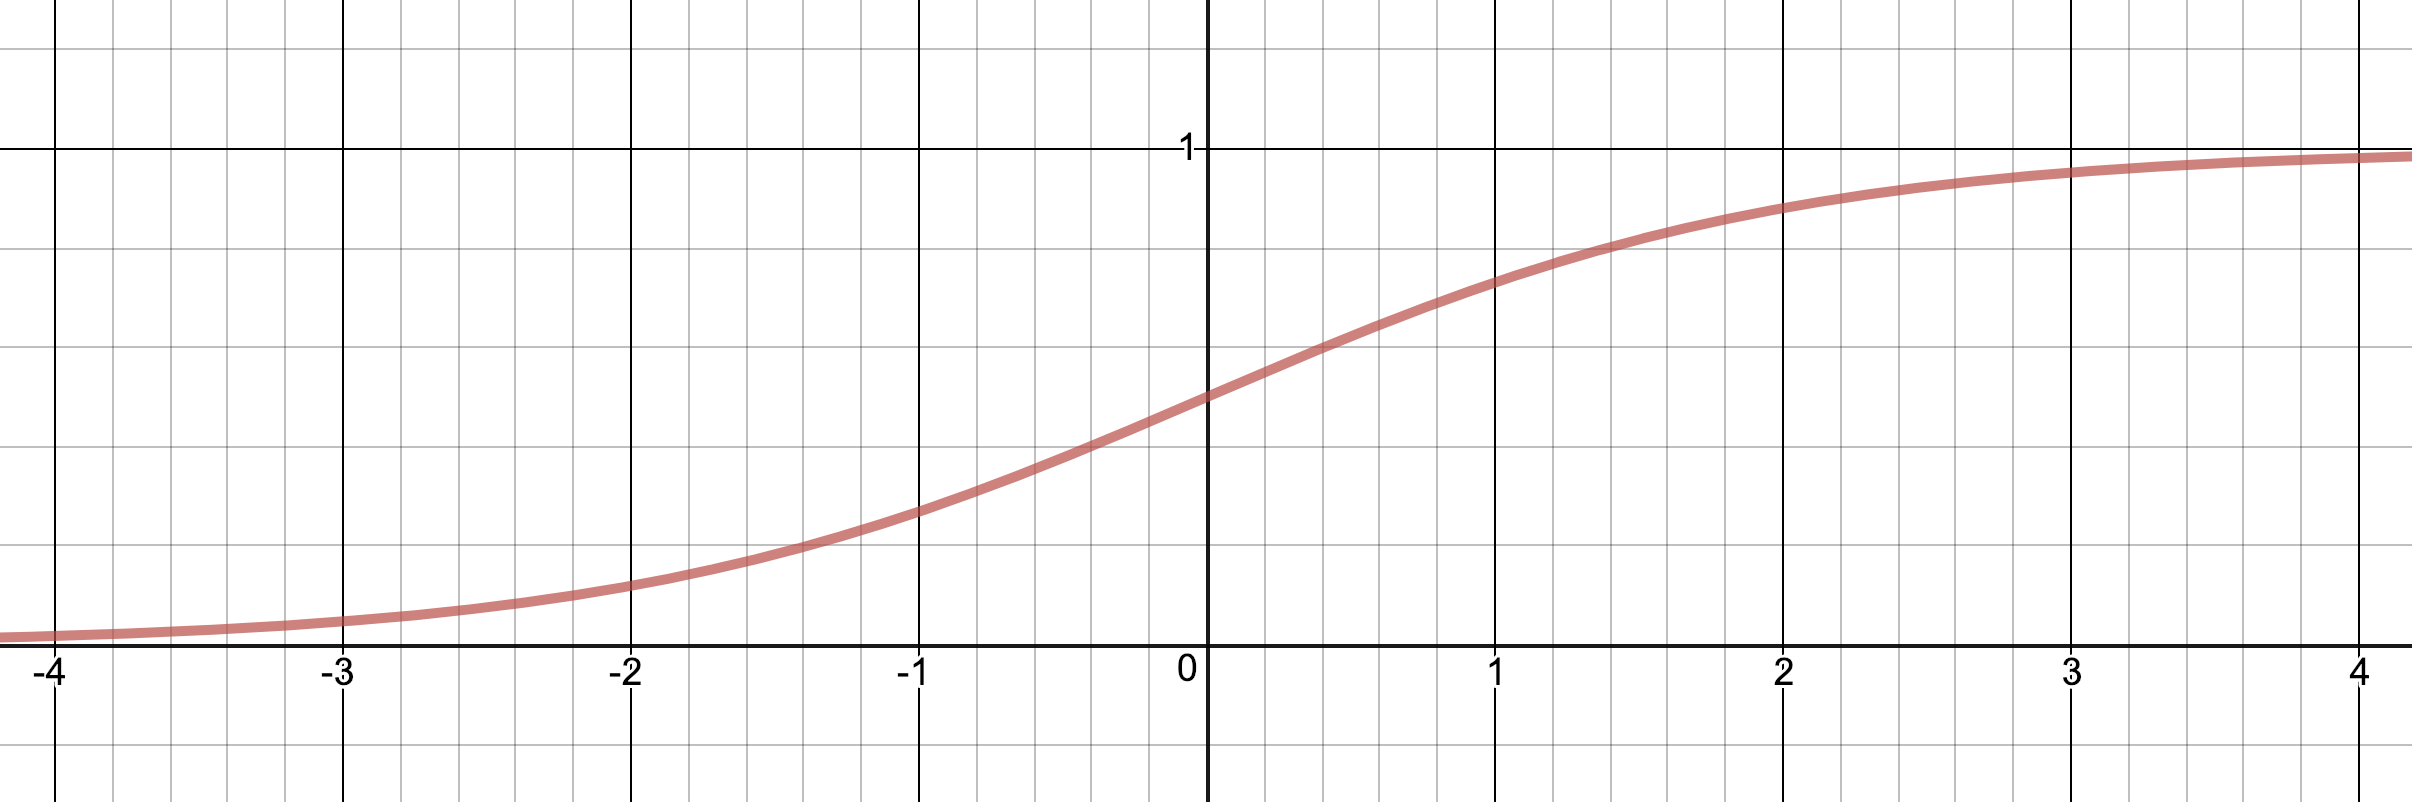
\includegraphics[scale=0.15]{sigmoid.png}
\end{center}

Classification function: $\widehat{f}_{\omega}(x) = \sigma(\omega x)$ with a threshold \\

\underline{Loss function}

If $y = 1$, we want $\sigma(\omega x)$ to be high => $1 - \sigma(\omega x)$ should be low. The loss function should be increasing with $1 - \sigma(\omega x) = 1 - \frac{1}{1+e^{-\omega x}} = \frac{1}{1+e^{\omega x}}$. Equivalently, it should be increasing with $1 + e^{-\omega x}$.

More generally, the loss function is defined as such: $\ell(f_{\omega}, (x,y)) = log(1 + e^{-y \omega x})$ (adding $y$ in the expression allows to take into account cases when $y = 1$ and $y = -1$).

Recall that the log is a monotonic function.

\vspace{5mm}

\underline{Estimation}

The advantage of the logistic loss function is that it is a convex function. Hence the ERM problem can be solved efficiently using santard methods.

Estimation is done using maximum likelihood. Maximum likelihood is finding the parameter that maximizes the probability to have a specific event $(x_i, y_i)$. We want to maximize the \textit{à posteriori} probability that depends on $x$: \\

$L(\omega, b) = \prod_{i=1}^n \pi(x_i)^{y_i}(1-\pi(x_i))^{1-y_i}$ \\

This equation has no analytic solution. We use a numeric method to find the optimal parameters (see optimizaton algorithms).

See \textit{Neural Network} section for more details on optimization.

\vspace{5mm}

Note: logistic regression is really a linear model since the objective is to find $\omega$ that is the slope of the line $\omega ^Tx + b$.

\vspace{5mm}